\beginsong{Piragenlagerlied}[mel={Die Opis}, txt={vom Piratenlager 2015 der Region Kurhessen}, index={Von der Strömung umspült}]

\markboth{\songtitle}{\songtitle}


\beginverse
\endverse

\centering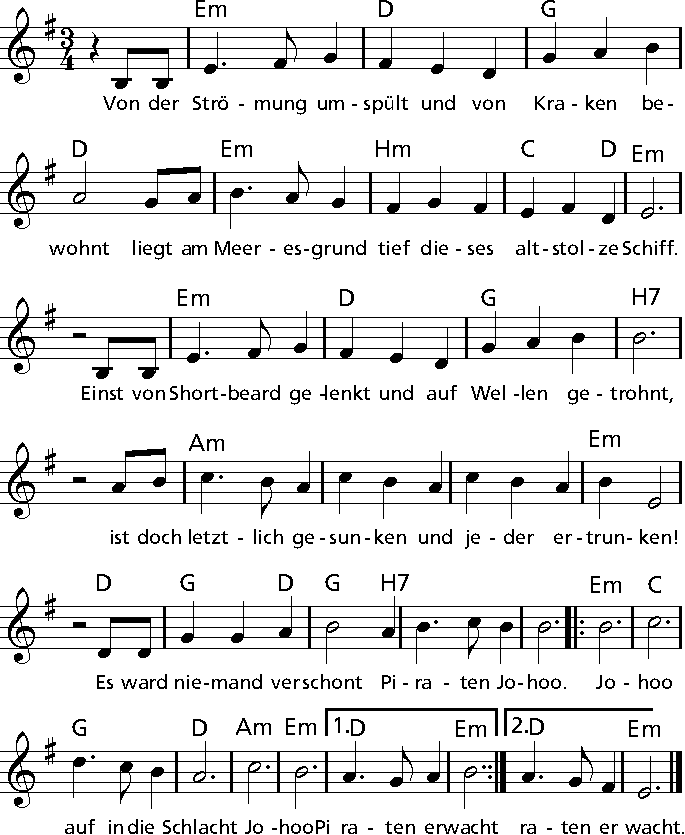
\includegraphics[width=1\textwidth]{Noten/Piratenlagerlied.pdf}	

\beginverse\memorize
Ihr \[Em]Freibeuter \[D]alle, nu \[G]kommet her\[D]bei
anzu\[Em]treten das \[D]Erbe des \[C]Königs \[D]der \[Em]See.
Ge\[Em]fahr und Ent\[D]behrung sind \[G]uns einer\[D]lei,
um den \[Am]stärksten zu finden und dann zu ent\[Em]schwinden,
\[D]so stimmt \[G]ein in den Schrei -- Pi\[H7]raten Johoo!
\endverse

\beginchorus
\lrep \[Em]Jo\[C]hoo, Pir\[G]aten er\[D]wacht, \[Am]jo\[Em]hoo, \[D]auf in die \[Em]Schlacht! \rrep
% \newline
\endchorus
%
% \centering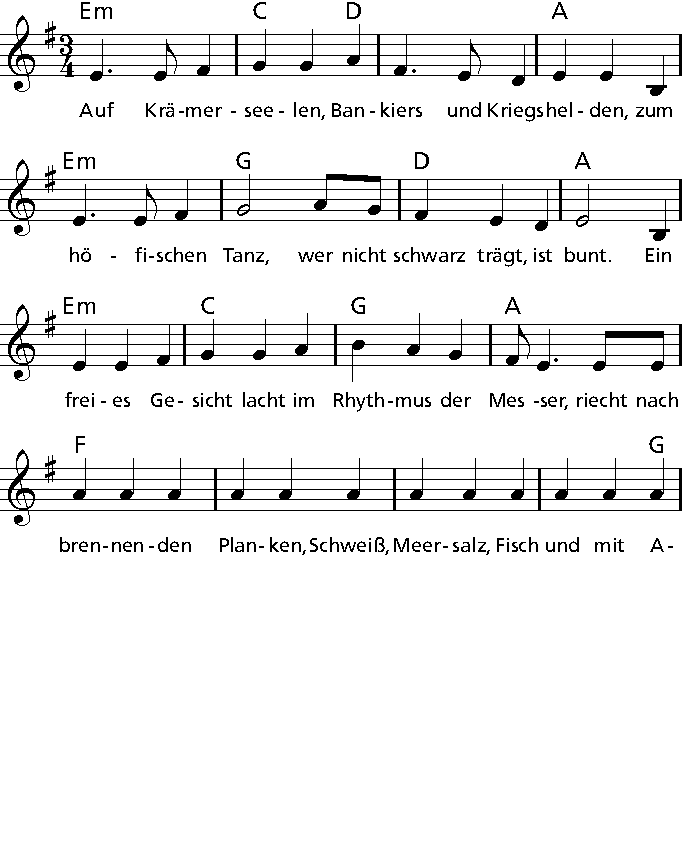
\includegraphics[width=1\textwidth]{Noten/Piratenlied_1a2.pdf}
% \newpage
%
% \centering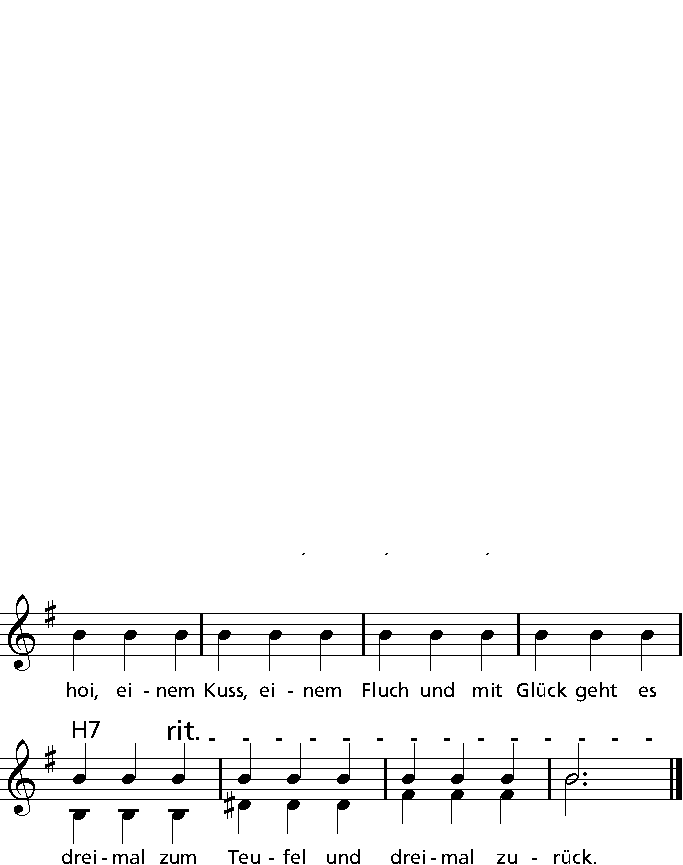
\includegraphics[width=1\textwidth]{Noten/Piratenlied_1b2.pdf}

% \beginverse
% \[Em]Auf Krämer\[C]seelen, Ban\[D]kiers und Kriegs\[A]helden.
% Zum \[Em]höfischen \[C]Tanz -- wer nicht \[D]schwarz trägt ist \[A]bunt.
% Ein \[Em]freies Ge\[C]sicht lacht im \[G]Rhythmus der \[D]Messer.
% Riecht nach \[F]brennenden Planken, Schweiß, Meersalz, Fisch und mit \[G]Ahoi, einem Kuss, einem Fluch und mit Glück geht es \[H7]dreimal zum Teufel und dreimal zurück.
% \endverse
%
% \beginchorus
% \lrep \[Em]Jo\[C]hoo, \[G]grüßet uns \[D]froh, \[Am]jo\[Em]hoo, \[D]fern Fala\[Em]do! \rrep
% \endchorus
%
% \beginverse
% Brüder ^trinkt auf die ^See, die uns ^ruft weit hi^naus,
% Aller ^Sünder Weg ^treiben wir ^ins nir^gend^wo,
% Kehrt doch ^keiner von ^unseren ^Fahrten nach ^Haus.
% Und so ^trinkt auf dies Leben, das bleibt un^vergeben!
% ^Und zum ^Ende trinkt aus -- Pi^raten Johoo!
% \endverse

% \beginchorus
% \lrep \[Em]Jo\[C]hoo, \[G]grüßet uns \[D]froh, \[Am]jo\[Em]hoo, \[D]fern Fala\[Em]do! \rrep
% \endchorus
%

\endsong

\beginscripture{}

\endscripture

\begin{intersong}

\end{intersong}